\documentclass{beamer}

\usepackage[utf8]{inputenc}
\usepackage{fontspec}
\usetheme{metropolis}
\usepackage{graphicx}


\setsansfont[BoldFont={Fira Sans}]{Fira Sans Light}
%\setsansfont[BoldFont={Fira Sans}]{Fira Sans Light}
\setmonofont{Fira Mono}
%\usetheme{default}

\title{Keeping Clients Synchronized}
\author{Michael Jonathan Lee}
\institute{FH Kiel}
\date{2018}

\begin{document}

\maketitle

\section{Single Client Scenario}

\begin{frame}
    \centering
    How can we ensure backend and client to stay synchronized?
\end{frame}

\begin{frame}
    \centering
    What do we mean by synchronized?
\end{frame}

\begin{frame}
    \frametitle{Definition of Synchronized}

    \begin{block}{client idle on the network}
        At a given time $t$ client has no pending or queued network requests.
    \end{block}

    \begin{block}{client up to date}
        At a given time $t$ the partial copy of server state in the Client
        is identical to the corresponding state on the server.
    \end{block}

    \begin{block}{client synchronized}
        At any time $t$ at which the client is idle on the network, the client
        is up to date.
    \end{block}
\end{frame}

\begin{frame}
    \centering
    Why can the client not be synchronized?
\end{frame}

\begin{frame}
    \centering
    Event with an idealized theoretical backend we can break things...
\end{frame}

\begin{frame}
    \frametitle{Backend}
    \centering
    \begin{block}{ideal backend}
        responds to requests in the same order it received those requests
    \end{block}
    \begin{block}{real backend}
        guarantees no ordering of requests and responses
    \end{block}
\end{frame}

\begin{frame}
    \frametitle{Requests}
    \begin{itemize}
        \item default backend communication is done via HTTP requests
        \item HTTP is stateless
        \item we have to issue requests asynchronously, to avoid the app from
            freezing
        \item the physical network connection has letency and package transfer
            times differ for a lot of reasons
    \end{itemize}
\end{frame}

\begin{frame}
    \frametitle{The Example App}
    Consider a simple app with just a single text input containing one character:

    \begin{itemize}
        \item the input represents a single state value in the backend
        \item the user can alter this value through the input
        \item every change the user makes is immediatly sent to the backend
    \end{itemize}
\end{frame}

\begin{frame}
    \centering
    So now our user very rapidly types A followed by B...
    \newline
    \newline
    ...which he expects to result in seeing B on his screen and beeing stored in
    the backend
\end{frame}

\begin{frame}
    \frametitle{broken 1}

    \begin{block}{arrival at server in order}
        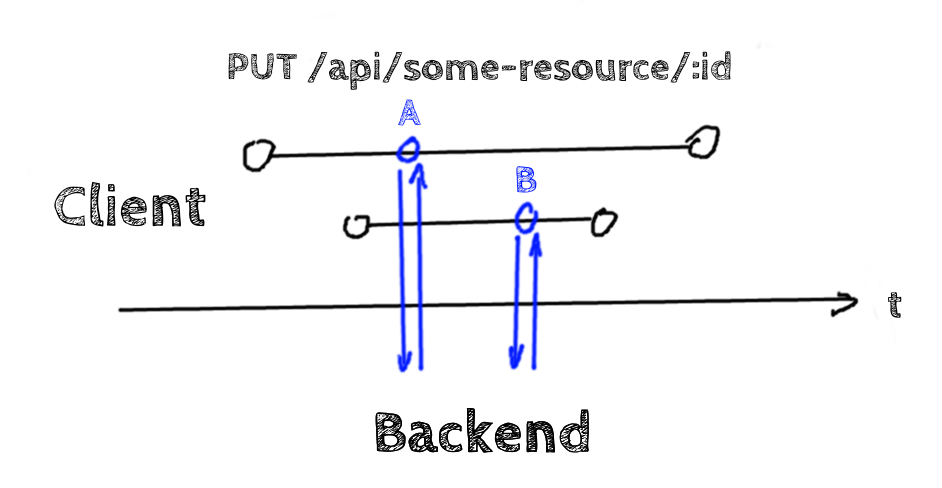
\includegraphics[scale=0.2]{right-result-wrong-sync}
        The server state is B as expected but the client state is A.
    \end{block}
\end{frame}

\begin{frame}
    \frametitle{broken 2}

    \begin{block}{arrival at server out of order}
        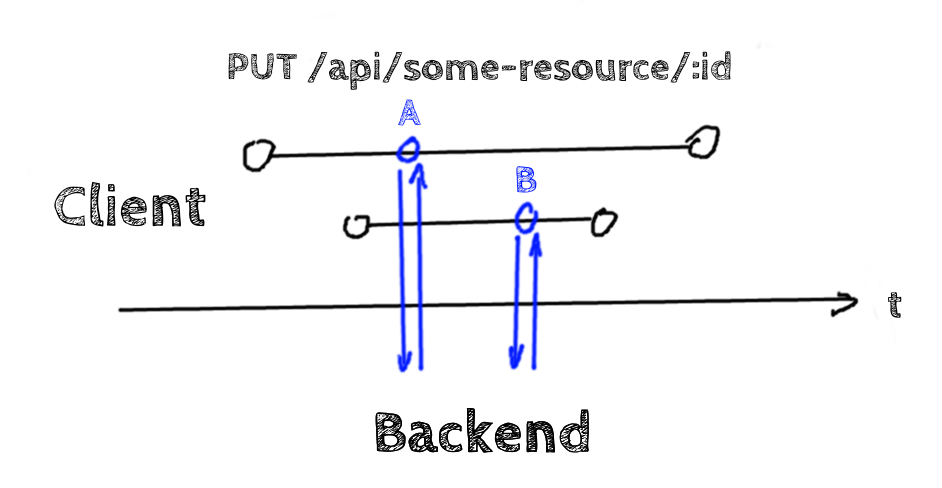
\includegraphics[scale=0.2]{right-result-wrong-sync}
        The server state has unexpected value A, but the client state is B.
    \end{block}
\end{frame}

\begin{frame}
    \centering
    Every example we have considered in this class so far is broken for simplicity!
\end{frame}

\begin{frame}
    \centering
    To fix this using traditional AJAX the client needs to define a lock state
    for any backend state it holds, to prevent it from sending double requests...
\end{frame}

\begin{frame}
    \frametitle{Drawbacks}
    \begin{itemize}
        \item tideous
        \item often hard to identify which parts of the guy get locked
        \item single requests can affect multiple parts of the state
        \item with multi client use cases this does not help at all
    \end{itemize}
\end{frame}

\begin{frame}
    \frametitle{The Real Problem}
    If we take a closer look we can clearly see that the underlying problem in
    this case is the statelessness of the HTTP requests.

    Why are we working with stateless connections anyway?
    \begin{itemize}
        \item historic reasons
        \item simplicity for backend development
        \item scalability
    \end{itemize}
\end{frame}

\begin{frame}
    \centering
    So what if we had a statefull connection method for ordered bidirectional
    communication?
\end{frame}

\begin{frame}
    \centering
    WebSockets to the rescue!
\end{frame}

\section{Multiple Client Scenario}


\end{document}
